% IEEE PAPER FORMAT 
\documentclass[twocolumn,oneside,conference]
{IEEEtran}

%%%%%%% all the required packages are loaded%%%%
\usepackage{filecontents}
\usepackage[style=ieee,backend=biber]{biblatex}
\usepackage{graphicx}
\usepackage{lmodern}
\usepackage{enumerate}
\usepackage{float}

% bibilography page%%%%%%%%%%%%%%
\begin{filecontents}{Master.bib}
@proceedings{this123,
editor = {Sriharsha Harsha et al},
title = {This is a test paper},
year = {2016}
}
\end{filecontents}
%%%%%%%%%%%%%%%%%%%%%%%%%%%%%%%%%%%%%%%



\addbibresource{Master.bib}

\IEEEoverridecommandlockouts 
\renewcommand\IEEEkeywordsname{Keywords}


\title{ICNV-TV: A read-depth based Copy Number Variation detection tool}
\markboth{Journal of Not yet Decided}{Sriharsha \MakeLowercase{\textit{et al}}: A read-depth based Copy Number Variation detection tool}

\author{
	\IEEEauthorblockN{Sriharsha Vogeti} 
	\IEEEauthorblockA{CCNSB,IIIT-Hyderabad\\
	vogetisri.harsha@research.iiit.ac.in}
	\and
	\IEEEauthorblockN{Prashanthi D} 
	\IEEEauthorblockA{CCNSB,IIIT-Hyderabad\\
	prashanthi.d@research.iiit.ac.in}
	\and
	\IEEEauthorblockN{Nita Parekh} 
	\IEEEauthorblockA{CCNSB, IIIT-Hyderabad\\
	nita@iiit.ac.in}
	
}

\begin{document}
\maketitle


 
\begin{abstract}
Copy Number Variation (CNV) is a form of structural variation contributing significantly to variations found in human genomes. A number of studies, so far have shown that CNVs are associated with complex diseases. Micro-array genomic comparative hybridization   (arrayCGH)and fluorescence in situ hybridization (FISH) provided were limited by the low resolution offered. The advancement in sequencing technologies leading to the development of Next Generation Sequencing (NGS) techniques solved this problem by offering very high resolution. We develop a read-depth (RD) based pipeline called ICNVTV, having a total variation penalized least squares model for segmentation which was proposed by Duan et al 2013. A comprehensive testing, followed by comparison against other RD-based tools was done on simulated data and real data. We analysed results obtained from applying our method to five different populations belonging to South Asian region. Both the real data and population data were obtained from 1000Genome Project. \\
\end{abstract}
 
\begin{IEEEkeywords}
CNV Detection, CNVTV, Read-Depth Methods, Population Studies, NGS\\
\end{IEEEkeywords}
\section{Introduction}
\IEEEPARstart{S}ome shit \cite{this123}

\section{Methods}
General input description 
\subsection{Preprocessing}
\subsection{Segmentation}
\subsection{Postprocessing}

\section{Results}
Discussion about what has been done
\subsection{Simulated Data}
\subsection{Real Data Analysis}
\subsection{Sub-population Analysis}
\begin{figure*}[h]
	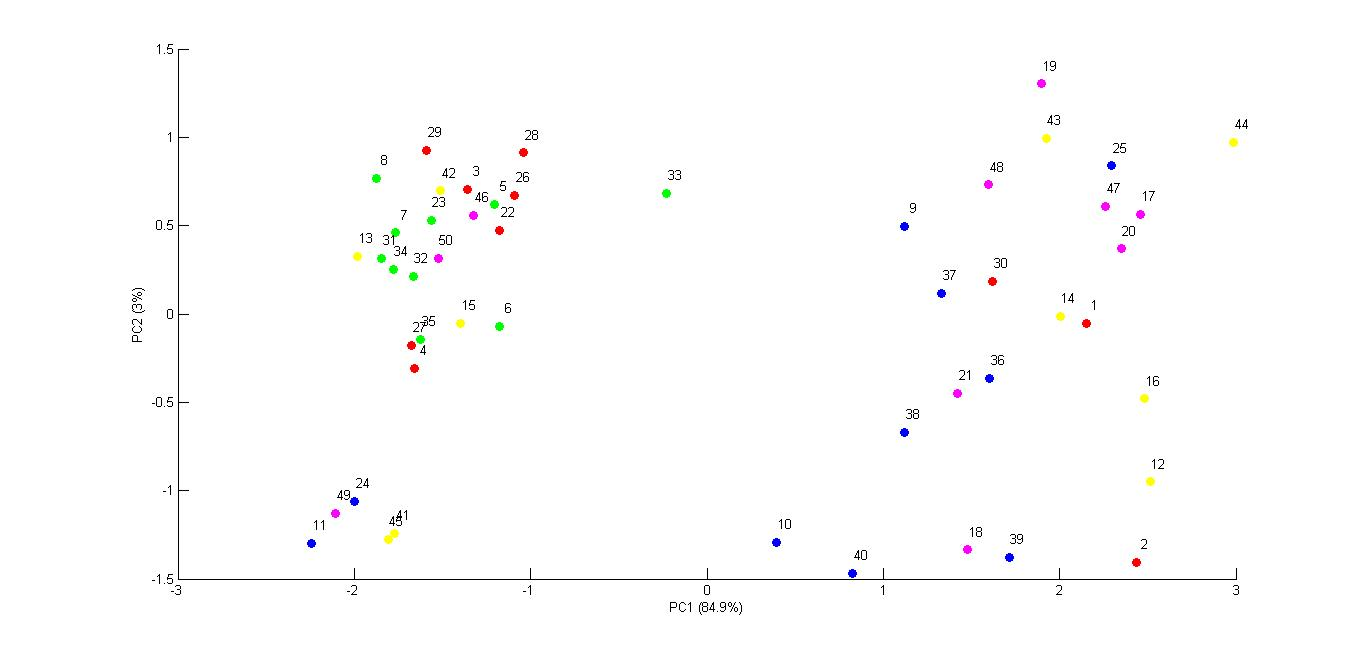
\includegraphics[width=\linewidth]{final.jpg}
	\caption{This is a test image}
	\label{fig1: this is test image}
\end{figure*}

\section{Discussion}

\section{Future work}

\section*{Acknowledgments}


\printbibliography

\end{document}



